%\documentclass[border=0.125cm]{standalone}
\documentclass{standalone}
\usepackage{tikz}
\usetikzlibrary{positioning}
\begin{document}
\tikzset{%
  every neuron/.style={
    circle,
    draw,
    minimum size=1cm
  },
  neuron missing/.style={
    draw=none, 
    scale=4,
    text height=0.333cm,
    execute at begin node=\color{black}$\vdots$
  },
}
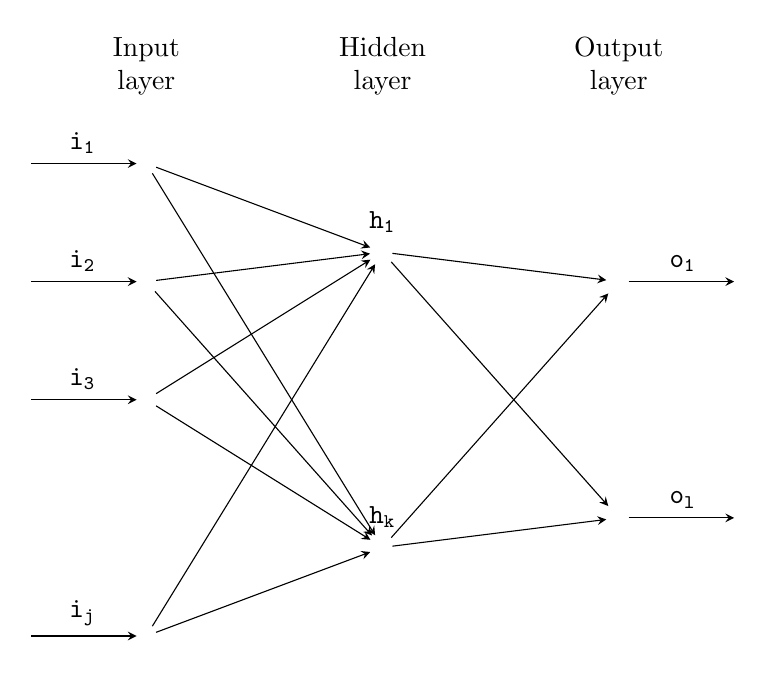
\begin{tikzpicture}[x=1.5cm, y=1.5cm, >=stealth, shorten >=1pt]
% Draw input nodes
\foreach \m/\l [count=\y] in {1,2,3,missing,4}
  \node [every neuron/.try, neuron \m/.try] (input-\m) at (0,2.5-\y) {};

% Label input nodes
\foreach \l [count=\i] in {1,2,3,j}
  \draw [<-] (input-\i) -- ++(-1,0)
  node [above, midway] {$\mathtt{i_\l}$};

% Draw hidden nodes
\foreach \m [count=\y] in {1,missing,2}
  \node [every neuron/.try, neuron \m/.try ] (hidden-\m) at (2,2-\y*1.25) {};

% Label hidden nodes
\foreach \l [count=\i] in {1,k}
\node [above] at (hidden-\i.north) {$\mathtt{h_\l}$};

% Draw output nodes
\foreach \m [count=\y] in {1,missing,2}
  \node [every neuron/.try, neuron \m/.try ] (output-\m) at (4,1.5-\y) {};


% Label output edges 
\foreach \l [count=\i] in {1,l}
  \draw [->] (output-\i) -- ++(1,0)
  node [above, midway] {$\mathtt{o_\l}$};

% Connect input nodes with hidden nodes
\foreach \i in {1,...,4}
  \foreach \j in {1,...,2}
    \draw [->] (input-\i) -- (hidden-\j);

% Connect hidden nodes with output nodes
\foreach \i in {1,...,2}
  \foreach \j in {1,...,2}
    \draw [->] (hidden-\i) -- (output-\j);

% Annotate the layers
\foreach \l [count=\x from 0] in {Input, Hidden, Output}
  \node [align=center, above] at (\x*2,2) {\l \\ layer};
\end{tikzpicture}
\end{document}
